\documentclass[a4paper,11pt]{article}
\usepackage{url}
\usepackage{hyperref}
\usepackage{listings}
\usepackage{color}
\usepackage{tikz}
\usetikzlibrary{arrows}
\usetikzlibrary{patterns}

\hoffset 0in
\oddsidemargin 0in
\voffset -0.4in
\topmargin 0in
\headheight 12pt
\headsep 0,5in

\marginparwidth 50pt
\marginparsep 5pt
\reversemarginpar


\textwidth 6.5in
\displaywidth 6.5in
\textheight 240mm
\parindent 0mm
\parskip \baselineskip

\newcommand{\code}[1]{\texttt{#1}}

%\newcommand{\heading}[1]{\vspace{2ex}\section*{#1}}
\newcommand{\refsection}[1]{Section \ref{#1}}


\begin{document}

\title{\bf ENEL464 Embedded Software and Advanced Computing 2025 \\ Group Assignment 2}
\author{}
%\author{Michael Hayes}
\date{}
\maketitle


\section{Introduction}

This is a group assignment with three students per group.

The purpose of this assignment is to implement a numerical algorithm
on a computer to make the most efficient use of its caches and cores.
You will find that you will get a large variation in program
performance depending on how you implement your code and use compiler
optimisations.  A knowledge of computer architecture should help with
this!

The algorithm is Jacobi relaxation.  This is an iterative algorithm
used to approximate differential equations, for example, Poisson's and
Laplace's equations.  Poisson's equation can be used to find the
electric potential given a specified charge distribution or
temperature given a specified heat source.  There are more efficient
ways to solve this problem using Green's functions and Fourier
transforms but that is not the purpose of this assignment.

\section{Jacobi relaxation}

The discrete form of Poisson's equation is
%
\begin{equation}
  \nabla^2 V_{i,j,k,n} = f_{i,j,k,n},
\end{equation}
%
where $f_{i,j,k_n}$ is the source for a voxel with coordinates $i,j,k$
at timestep $n$ and $V_{i,j,k,n}$ is the potential field to be
determined for the same voxel.  If $f$ is the source charge, $V$ is
the electric potential.

Poisson's equation is a partial differential equation and thus
requires boundary conditions to achieve a solution.  For the
assignment, the boundaries are the six sides of a cube.  The potential
on the left side ($i=0$) is -2\,V, the potential on the right side
($i=N-1$) is 1\,V, and the other four sides are insulated.  This is a
mixed boundary condition problem since two sides have Dirichlet
boundary conditions and the other sides have Neumann boundary
conditions.

Poisson's equation can be solved iteratively, at each time-step $n$,
using Jacobi relaxation, where\footnote{You might recognise
  (\ref{eqn:Jacobi}) as a 3-D discrete convolution at each time-step.}
%
\begin{equation}
  V_{i,j,k,n+1} = \frac{1}{6} \left(V_{i+1,j,k,n} + V_{i-1,j,k,n} + V_{i,j+1,k,n} + V_{i,j-1,k,n} + V_{i,j,k+1,n} + V_{i,j,k-1,n} - \Delta^2 f_{i,j,k}\right).
\label{eqn:Jacobi}
\end{equation}
%
Here $\Delta = \Delta x = \Delta y = \Delta z$ is the spacing between
voxels in metres, $0 \le i < N$, $0 \le j < N$, and $0 \le k < N$.

Voxels on the insulated boundaries are defined such that the
derivative over that boundary is zero ($\partial V / \partial n = 0$),
see Fig.~\ref{fig:Boundary}.  For example, consider the derivative in
the z-direction, $\partial V / \partial z$.  This can be approximated
by the central difference,
%
\begin{equation}
  \frac{V_{i,j,k+1} - V_{i,j,k-1}}{2\Delta}.
\end{equation}
%
On the boundary where $k=0$, then
%
\begin{equation}
  \frac{V_{i,j,1} - V_{i,j,-1}}{2\Delta},
\end{equation}
%
and for this to be zero implies $V_{i,j,-1} = V_{i,j,1}$.  Since these
voltages are the same, no current flows normal to the boundary as
expected for an insulating boundary.  Similarly, on the other opposite
boundary, $V_{i,j,N} = V_{i,j,N-2}$.


\begin{figure}
  \centering
  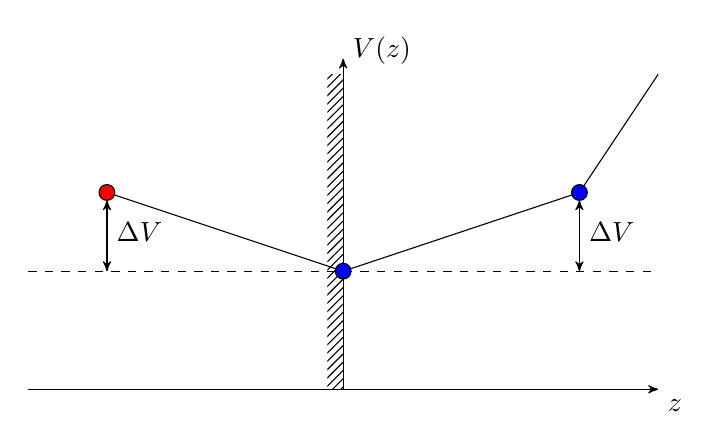
\begin{tikzpicture}
    \tikzset{>=stealth'}

    % Draw some axes
    \draw[->] (-4, 0) -- (4, 0);
    \draw[->] (0, 0) -- (0, 4.2);

    \node[above right] at(0, 4) {$V(z)$};
    \node[below right] at(4, 0) {$z$};

    % Draw the boundary
    \fill[pattern=north east lines]
        (-0.2, 0) -- (-0.2, 4) -- (0, 4) -- (0, 0);

    \draw (-3, 2.5) -- (0, 1.5) -- (3, 2.5) -- (4, 4);

    \draw[dashed] (-4, 1.5) -- (4, 1.5);

    \draw[fill=red] (-3, 2.5) circle (0.1);
    \draw[fill=blue] (0, 1.5) circle (0.1);
    \draw[fill=blue] (3, 2.5) circle (0.1);

    \draw[<->] (-3, 1.5) -- (-3, 2.4);
    \draw[<->] (3, 1.5) -- (3, 2.4);

    \node[right] at (3, 2) {$\Delta V$};
    \node[right] at (-3, 2) {$\Delta V$};
  \end{tikzpicture}
  \caption{Illustration of a Neumann boundary condition where the external
  `ghost' point (red) is defined such that the gradient at the boundary is zero
  with respect to the internal points (blue).}
  \label{fig:Boundary}
\end{figure}


\section{Implementation}

Your program to solve (\ref{eqn:Jacobi}) must either use C or C++.
Your goal is to find a fast implementation that will run on your (or
an ECE lab) computer, making best use of the caches and multiple
cores.

A good starting point is provided with \code{poisson.c}. You should
modify this to solve the assignment.  Instructions on building it are
in the repository README.  Some suggested reading is located in the
\emph{docs/} folder regarding compiler optimisations, multithreading,
and profiling.

Code templates can be found at
\url{https://eng-git.canterbury.ac.nz/mph/ence464-assignment-2025}. 
A fork of this repository will be given to you before your first lab.

We recommend writing your solutions in a Linux-like environment. This
means any Linux distribution, MacOS with Homebrew, or Windows with
WSL. Your mileage may vary with the profiling tools in anything other
than Linux.


\section{Testing}

Test your algorithm with a single point charge in the centre of the
volume, i.e.,
%
\begin{equation}
  f_{i,j,k} = \left\{
  \begin{array}{ll}
    1 & i=N/2, j=N/2, k=N/2, \\
    0 & \mbox{otherwise}
  \end{array}\right.,
\end{equation}
%
where the volume is comprised of $N \times N \times N$ voxels.  

You can also test it with an arbitrary source distribution described
by a set of coordinates in a text file. Instructions for the required
format can be found in the repository README.

A testing script (\code{test.sh}) has been provided along with some sample
outputs at several cube sizes and variable distributions. This will 
automatically compare your output against a reference implementation.

Once a correct solution has been implemented, rename
\code{gitlab-ci.yml} to \code{.gitlab-ci.yml} to enable gitlab continuous
integration. The pipeline will run your code against the reference
solutions to confirm the correctness of your algorithm. Please do not
attempt to use this for performance testing.

%% There is a simple explanation of the 2-D algorithm at
%% \url{https://blogs.msdn.microsoft.com/visualizeparallel/2010/03/29/the-jacobi-relaxation-an-instance-of-data-parallelism/}

\section{Support}

Only questions submitted via the ENCE464 assignment forum will be
answered.  Emails will be quietly ignored.


\section{FAQ}

\begin{itemize}
\item \emph{How do I find out the CPU version?}  Run \code{lscpu}.
  You can also run \code{lshw} but this needs root privileges to get
  the cache sizes.  Note, Linux considers each thread of a
  multithreaded core to be a CPU.

\item \emph{Why is my program killed?}  This is due to the Linux out
  of memory killer; you have tried to allocate too much memory.

\end{itemize}



\section{Reports}

The reports are to be submitted as PDF documents through the ENCE464 
Learn page.  They will be submitted to TurnItIn for plagiarism checking.
Use the supplied templates in the \code{docs/} folder and follow the 
instructions within.

Guidelines for writing a report are available
at\\ \url{https://eng-git.canterbury.ac.nz/mph/report-guidelines/blob/master/report-guidelines.pdf}.
However, no titlepage, abstract, introduction, or conclusion are
required.


\section{Assessment}

The marks breakdown is:
\begin{flushleft}
  \begin{tabular}{|l|r|}
    \hline
    Item        & Proportion\\
    \hline
    Group report        & 70\%\\
    Individual report   & 30\%\\
    \hline
    Benchmarking (bonus)& 5\%\\
    \hline
    \hline
    Total               & 100\%\\
    \hline
  \end{tabular}
\end{flushleft}

The group report will include the following sections:

\begin{itemize}
\item \textbf{Architecture overview}:  This should describe your computer's
  architecture (such as the cache organisation, memory size, CPU model,
  etc.).

\item \textbf{Multithreading analysis}:  This should discuss how your program
  takes advantage of multiple cores.

\item \textbf{Cache analysis}:  This should discuss how your program takes
  advantage of the cache.

\item \textbf{Optimisation analysis}:  This should discuss the affects of some
  of the compiler optimisations, such as loop unrolling, on your
  program.
\end{itemize}

The individual report will include the following sections:
\begin{itemize}
\item \textbf{Individual topic}:  This should address an aspect of computer
  architecture related to the assignment.  For example, using SIMD
  instructions, using the GPU, comparing two different computers,
  analysing branch prediction, optimisation, profiling, caching
  etc. in more detail.  Since this is an individual assessment,
  the work must be completed individually, and duplicated work 
  will be considered plagiarism.
\item \textbf{Contribution statement}:  A brief bullet-point
list of contributions you've made to the group aspect of the project.
\end{itemize}

In addition to the quality of the content, both group and individual 
reports will be marked on:
\begin{itemize}
\item \textbf{Written style}:  The writing should be concise technical writing.

\item \textbf{Presentation}:  The key here is consistency and clear diagrams
  and graphs.
\end{itemize}


Your reports should present the statistics for the time your program
takes to run for the following problem sizes: $N=101, 201, 301, 401,
501, 601, 701, 801, 901$.  For $N=801$ and $N=901$, do not worry about
performing many trials.  If you have a really old computer, you can
skip $N=901$.

Your analyses should be backed up with experimental evidence, such as
the output from profiling tools.

Bonus marks will be awarded to any group who can beat our (not
very good) program when running on a pre-specified ESL lab computer
and give the correct results.  We will reveal the computer a week
before the benchmarking trials.  Refer to Section \ref{code} for 
more details.

\section{Code} \label{code}

We require you to use git for version control.  We will look at your
code if we suspect plagiarism.

Your fastest implementation must be an executable named \code{poisson}
that is built by running \code{make} at the command line.  For testing
purposes, it must accept the following command line flags:
\begin{itemize}
  \item \code{-n}: the edge length of the cube.
  \item \code{-i}: the number of iterations.
  \item \code{-s}: the path/name of the file containing coordinates 
  for the source distribution. Your program should default to a source
  point with an amplitude of 1.0 at the center of the cube if this argument 
  is not provided.
  \item \code{-t}: the number of threads to run. Your program should default 
  to the optimal number of threads when this argument is not provided.
\end{itemize}
Your program must print out the resulting values from the middle slice of the
cube in space-separated format to five decimal places.  (You can just
use the command line argument parsing and output formatting code in
the provided \code{main.c}). For the benchmarking competition you must
use \textbf{doubles}.


\section{AI}

You are permitted to use generative artificial intelligence (AI) to
assist you in any way within the bounds of academic integrity. You
must appropriately acknowledge any use of generative AI in your
work. Please include a statement of acknowledgment with your work,
clearly indicating which AI tools were used and how they contribute to
your assessment.

\end{document}
